\chapter{Evaluation}\label{chap:evaluation}
	In this part of this thesis the models and methods outlined in the project will be evaluated. As outlined in the previous chapter, an experimentation interface was built to parametrize the assembly of the dataset and use different learning machines for each parameterization. First, the data will be extracted as it is in the xml-files and then then gradually this parametrization will be tweaked to evaluate the used methods in this thesis and gauge the performance enhancement through using them. This chapter with be divided into two main parts. Firstly, the vanilla learning machines that build a one-to-one relationship will be evaluated. Next, recurrent neural models will be examined and evaluated. This evaluation is by no mean an exhaustive use of the experimentation interface and only provide an insight to each use case, where a significant increase of performance was observed. This is mainly due to the complexity of training recurrent neural networks, which in average takes between three hours for four epochs.\newline
	In fig \ref{fig:vis_example} the interface of the visualisation of the results for each fold is shown, where tabs are used to separate the results of each experiment in the experiment set.
	\begin{figure}[H]
		\centering
		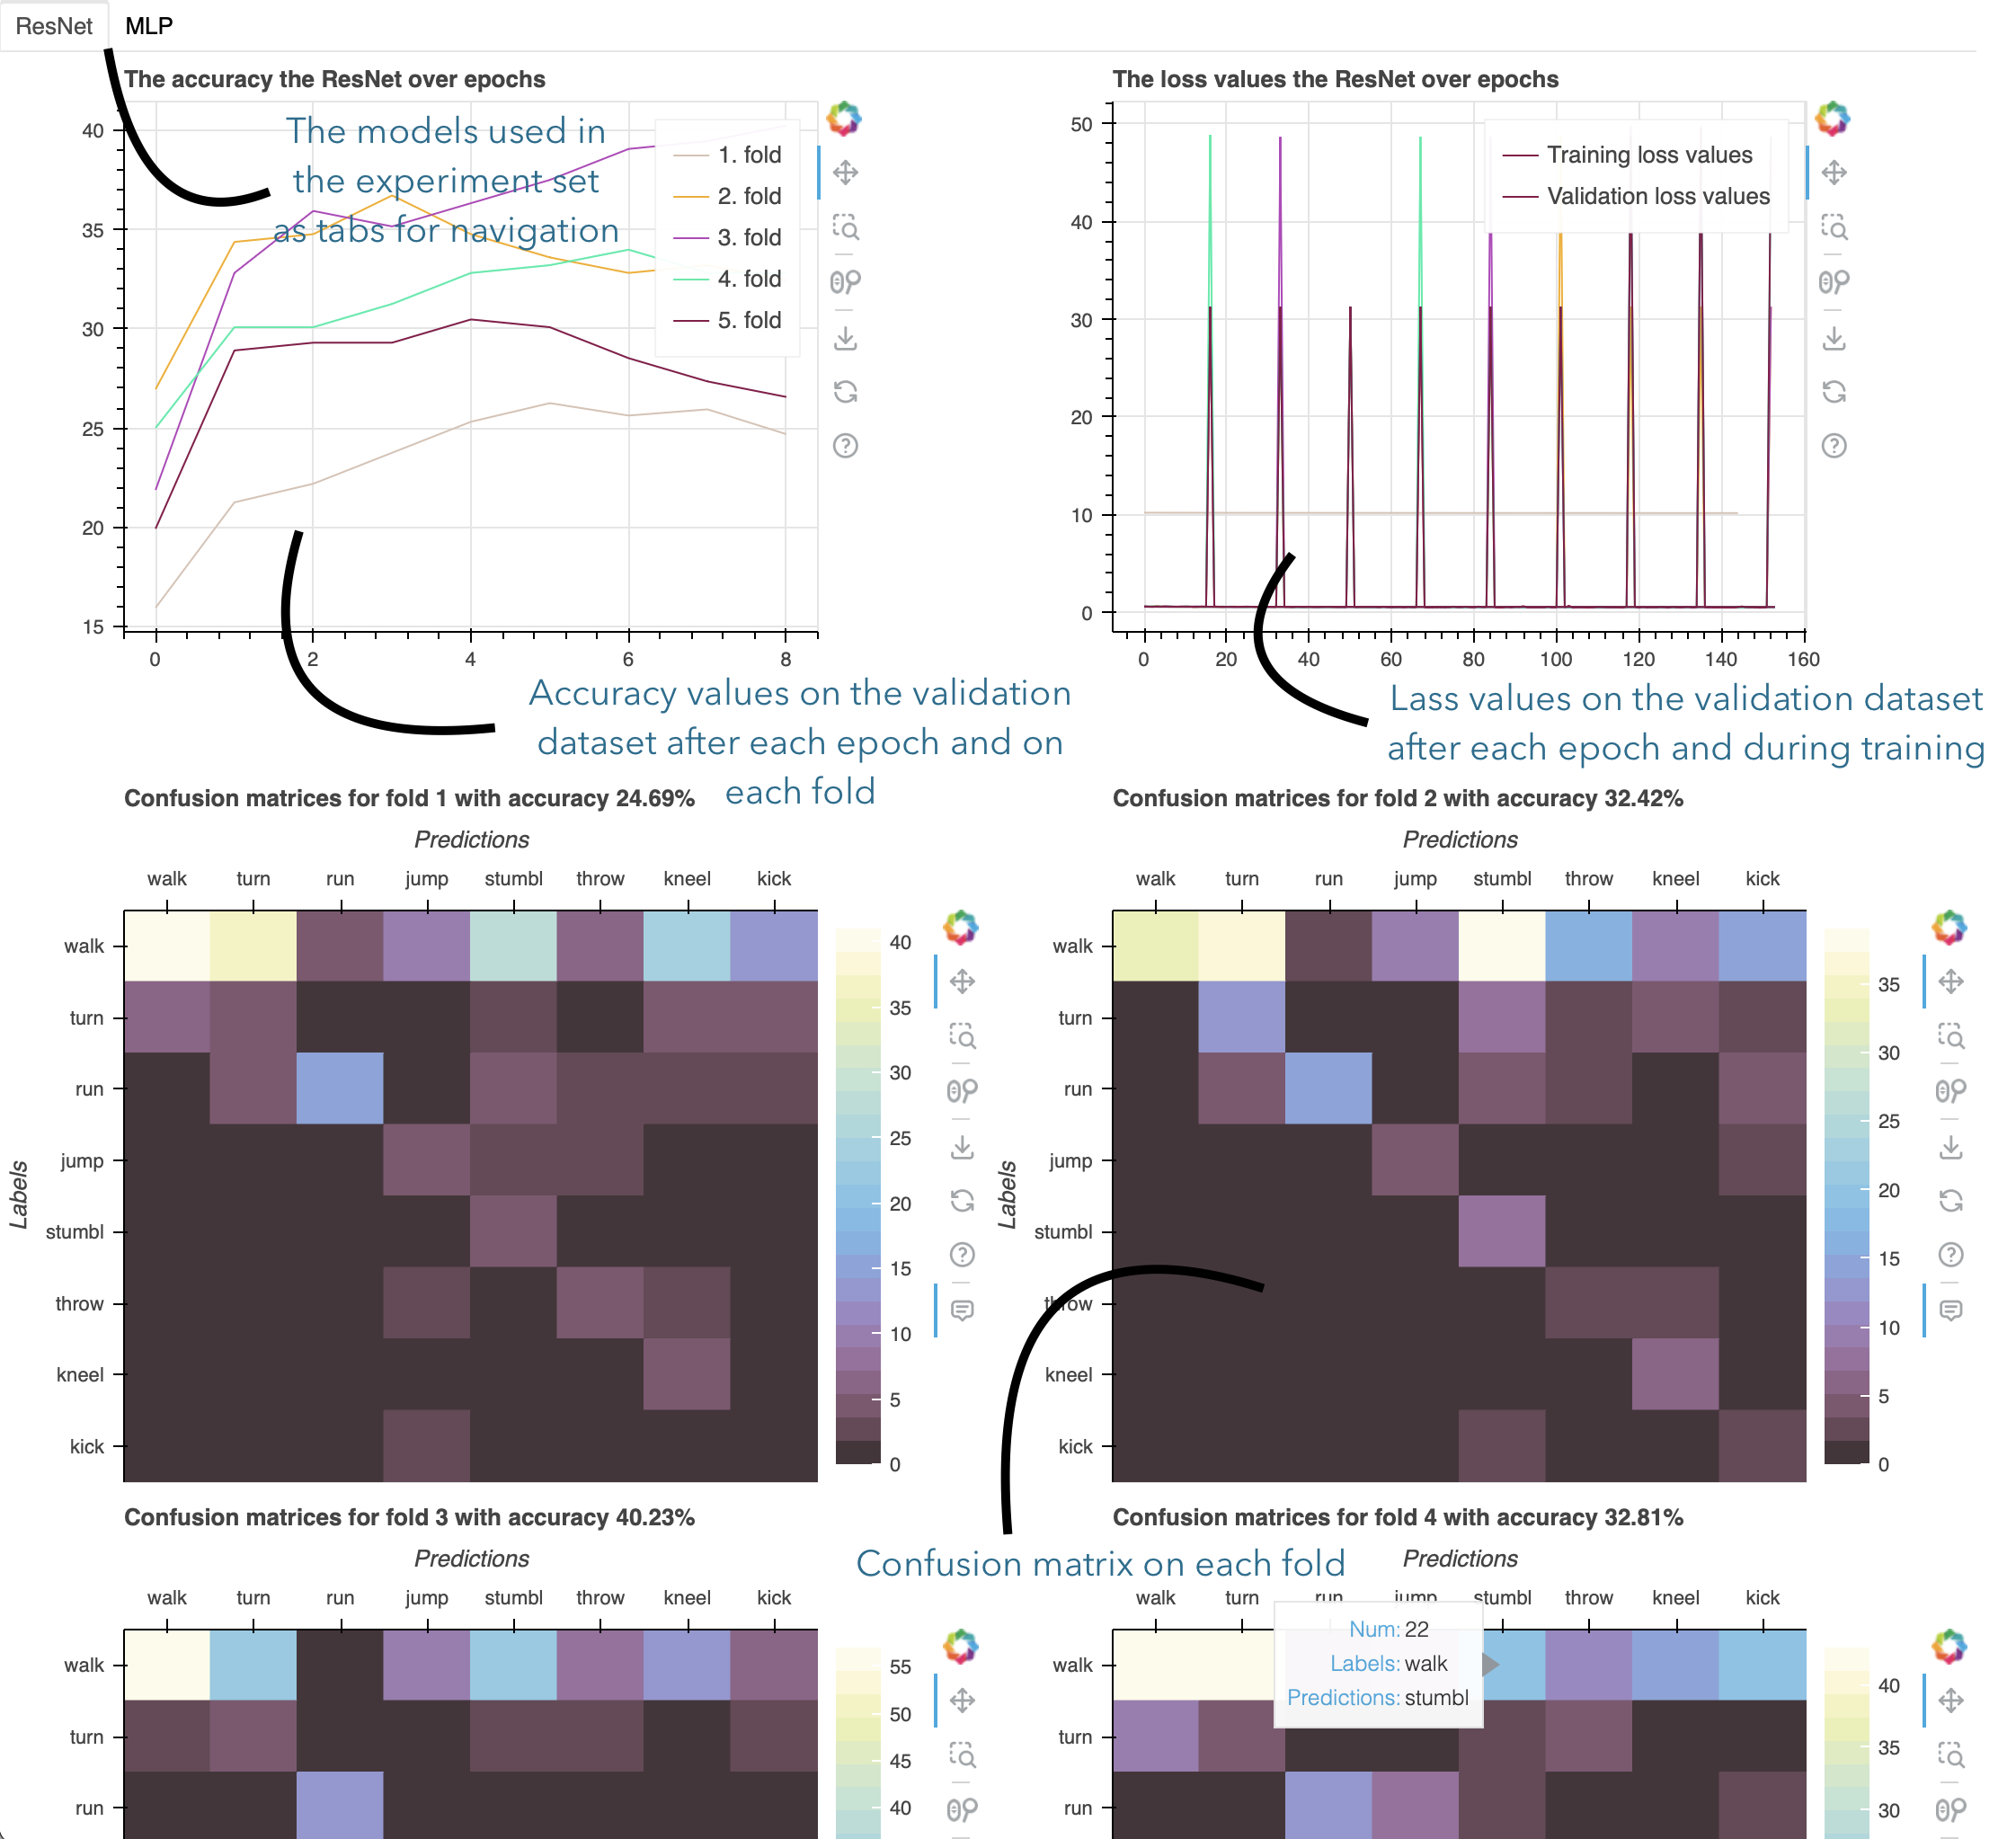
\includegraphics[width=\textwidth]{img/the-interface-of-the-visualisation-of-the-results-for-each-experiment-set.png}
		\caption{The interface of the visualisation of the results for each experiment set}
		\label{fig:vis_example}
	\end{figure}
	\section{One-to-one learning machines}\label{subsec:eva_one2one} 
		For this section the following learning machines will be used:
		\begin{itemize}
			\item MLP
			\item CNN
			\item FCN
			\item ResNet
		\end{itemize}
		In summery, these model proved to be very resilient and without oversampling it performed very well in comparison to sequence modelling learning machines. However, due to the use of the weighted loss function instances of the \textbf{walk} class were greatly misclassified in comparison to other models. The culprit here is the inter-class similarity, where the learning machines find it hard to find and learn good features for each class. In addition to that, the loss value for the validation sets plateaus after few epochs. This also the case for the loss values during the training, where after taking the first batches in the training set the loss values swing in a small interval and plateau after four or five epochs. 
		\subsection{Naive Approach}
			First, lets take the data stored in xml-file without normalization or oversampling to see, if these offer any advantage and check in which case this might be detrimental to the overall performance of the trained learning machines. Taking different parameters into account can establish a relationship between good features and good representation of each class of motions.\newline
		\subsection{Normalization}
		\subsection{Oversampling}
		\subsection{Normalization+Oversampling}
		\subsection{Reduce the Number of frames}
	\section{Sequence modelling learning machines}
		For this section the following learning machines will be used:
		\begin{itemize}
			\item RNN
			\item GRU
			\item LSTM
		\end{itemize}
		In summery, these models offered less or no performance compared to learning machines in \ref{subsec:eva_one2one} and seem to perform poorly for all data, i.e. root information, joint position and the combination of both. This proves that these models are incompatible with the data extracted from the xml-files. As mentioned in the introductory part of this chapter. Training these models is very difficult and require a lot of resources, thus making the training with more epochs prohibitive and time-consuming. 
		\subsection{Naive Approach}
		\subsection{Normalization}
		\subsection{Oversampling}
		\subsection{Normalization+Oversampling}
		\subsection{Reduce the Number of frames}
